\section{4 de febrero de 2021}

\begin{definition}
\begin{center}
    

\tikzset{every picture/.style={line width=0.75pt}} %set default line width to 0.75pt        

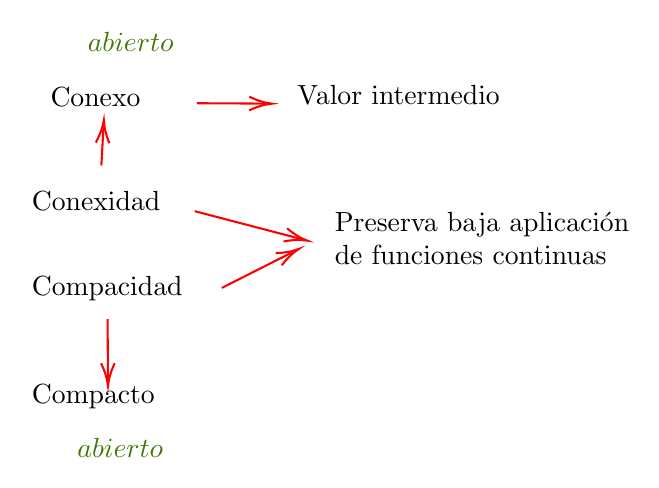
\begin{tikzpicture}[x=0.75pt,y=0.75pt,yscale=-1,xscale=1]
%uncomment if require: \path (0,300); %set diagram left start at 0, and has height of 300

%Straight Lines [id:da5220143812109725] 
\draw [color={rgb, 255:red, 255; green, 0; blue, 0 }  ,draw opacity=1 ]   (122,146) -- (122.19,176.2) ;
\draw [shift={(122.2,178.2)}, rotate = 269.64] [color={rgb, 255:red, 255; green, 0; blue, 0 }  ,draw opacity=1 ][line width=0.75]    (10.93,-3.29) .. controls (6.95,-1.4) and (3.31,-0.3) .. (0,0) .. controls (3.31,0.3) and (6.95,1.4) .. (10.93,3.29)   ;
%Straight Lines [id:da9488864909412285] 
\draw [color={rgb, 255:red, 255; green, 0; blue, 0 }  ,draw opacity=1 ]   (119,72) -- (120.09,52.2) ;
\draw [shift={(120.2,50.2)}, rotate = 453.15] [color={rgb, 255:red, 255; green, 0; blue, 0 }  ,draw opacity=1 ][line width=0.75]    (10.93,-3.29) .. controls (6.95,-1.4) and (3.31,-0.3) .. (0,0) .. controls (3.31,0.3) and (6.95,1.4) .. (10.93,3.29)   ;
%Straight Lines [id:da16251395696621607] 
\draw [color={rgb, 255:red, 255; green, 0; blue, 0 }  ,draw opacity=1 ]   (164,94) -- (216.27,107.69) ;
\draw [shift={(218.2,108.2)}, rotate = 194.68] [color={rgb, 255:red, 255; green, 0; blue, 0 }  ,draw opacity=1 ][line width=0.75]    (10.93,-3.29) .. controls (6.95,-1.4) and (3.31,-0.3) .. (0,0) .. controls (3.31,0.3) and (6.95,1.4) .. (10.93,3.29)   ;
%Straight Lines [id:da03666972810090552] 
\draw [color={rgb, 255:red, 255; green, 0; blue, 0 }  ,draw opacity=1 ]   (177,131) -- (212.41,113.1) ;
\draw [shift={(214.2,112.2)}, rotate = 513.19] [color={rgb, 255:red, 255; green, 0; blue, 0 }  ,draw opacity=1 ][line width=0.75]    (10.93,-3.29) .. controls (6.95,-1.4) and (3.31,-0.3) .. (0,0) .. controls (3.31,0.3) and (6.95,1.4) .. (10.93,3.29)   ;
%Straight Lines [id:da5243518205926371] 
\draw [color={rgb, 255:red, 255; green, 0; blue, 0 }  ,draw opacity=1 ]   (165,42) -- (199.2,42.19) ;
\draw [shift={(201.2,42.2)}, rotate = 180.32] [color={rgb, 255:red, 255; green, 0; blue, 0 }  ,draw opacity=1 ][line width=0.75]    (10.93,-3.29) .. controls (6.95,-1.4) and (3.31,-0.3) .. (0,0) .. controls (3.31,0.3) and (6.95,1.4) .. (10.93,3.29)   ;

% Text Node
\draw (93,32.9) node [anchor=north west][inner sep=0.75pt]   [align=left] {Conexo};
% Text Node
\draw (84,82.9) node [anchor=north west][inner sep=0.75pt]   [align=left] {Conexidad};
% Text Node
\draw (84,123.9) node [anchor=north west][inner sep=0.75pt]   [align=left] {Compacidad};
% Text Node
\draw (84,175.9) node [anchor=north west][inner sep=0.75pt]   [align=left] {Compacto};
% Text Node
\draw (106,202.1) node [anchor=north west][inner sep=0.75pt]  [color={rgb, 255:red, 65; green, 117; blue, 5 }  ,opacity=1 ]  {$abierto$};
% Text Node
\draw (111,6.1) node [anchor=north west][inner sep=0.75pt]  [color={rgb, 255:red, 65; green, 117; blue, 5 }  ,opacity=1 ]  {$abierto$};
% Text Node
\draw (230,92.9) node [anchor=north west][inner sep=0.75pt]   [align=left] {Preserva baja aplicación \\de funciones continuas};
% Text Node
\draw (212,31.9) node [anchor=north west][inner sep=0.75pt]   [align=left] {Valor intermedio};


\end{tikzpicture}
\end{center}
\end{definition}

\begin{remark}
$A$ es conexo, si $A$ no es disconexo. \newline 
\textbf{Disconexo:}
\begin{center}
    

\tikzset{every picture/.style={line width=0.75pt}} %set default line width to 0.75pt        

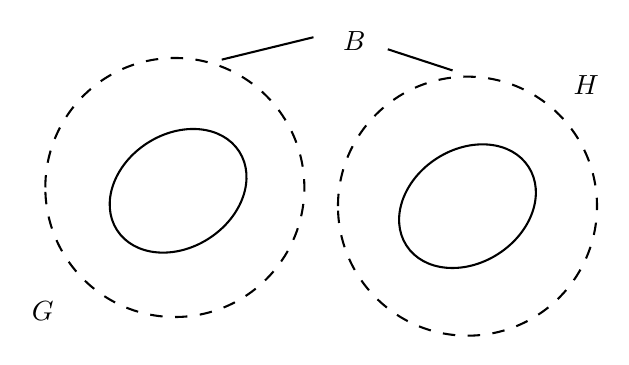
\begin{tikzpicture}[x=0.75pt,y=0.75pt,yscale=-1,xscale=1]
%uncomment if require: \path (0,300); %set diagram left start at 0, and has height of 300

%Shape: Circle [id:dp8455402914572695] 
\draw  [dash pattern={on 4.5pt off 4.5pt}] (100,94.6) .. controls (100,60.14) and (127.94,32.2) .. (162.4,32.2) .. controls (196.86,32.2) and (224.8,60.14) .. (224.8,94.6) .. controls (224.8,129.06) and (196.86,157) .. (162.4,157) .. controls (127.94,157) and (100,129.06) .. (100,94.6) -- cycle ;
%Shape: Circle [id:dp43487142688104174] 
\draw  [dash pattern={on 4.5pt off 4.5pt}] (241,103.6) .. controls (241,69.14) and (268.94,41.2) .. (303.4,41.2) .. controls (337.86,41.2) and (365.8,69.14) .. (365.8,103.6) .. controls (365.8,138.06) and (337.86,166) .. (303.4,166) .. controls (268.94,166) and (241,138.06) .. (241,103.6) -- cycle ;
%Shape: Ellipse [id:dp9061110877616693] 
\draw   (134.52,115.1) .. controls (126.36,102.38) and (132.93,83.61) .. (149.2,73.17) .. controls (165.46,62.73) and (185.26,64.57) .. (193.43,77.28) .. controls (201.59,89.99) and (195.02,108.76) .. (178.75,119.21) .. controls (162.48,129.65) and (142.68,127.81) .. (134.52,115.1) -- cycle ;
%Shape: Ellipse [id:dp419797908656945] 
\draw   (273.95,122.51) .. controls (265.79,109.8) and (272.36,91.03) .. (288.62,80.58) .. controls (304.89,70.14) and (324.69,71.98) .. (332.85,84.69) .. controls (341.01,97.4) and (334.44,116.17) .. (318.18,126.62) .. controls (301.91,137.06) and (282.11,135.22) .. (273.95,122.51) -- cycle ;
%Straight Lines [id:da9933913068723642] 
\draw    (185,33) -- (229.2,22.2) ;
%Straight Lines [id:da26845766244024405] 
\draw    (265,28) -- (296.2,38.2) ;

% Text Node
\draw (353,39.1) node [anchor=north west][inner sep=0.75pt]    {$H$};
% Text Node
\draw (92,148.1) node [anchor=north west][inner sep=0.75pt]    {$G$};
% Text Node
\draw (242,18.1) node [anchor=north west][inner sep=0.75pt]    {$B$};


\end{tikzpicture}
\end{center}

Si existen $G$ y $H$ (Disconexión de $B$) $\ni$
\begin{enumerate}
    \item $G\cap B\neq \emptyset$ y $H\cap B\neq \emptyset$
    \item $(G\cap B)\cap (H\cap B)=\emptyset$
    \item $(G\cap B)\cup (H\cap B)=B$
\end{enumerate}
\end{remark}

\begin{example}
\begin{enumerate}
    \item $\mathbb{Z}$ es disconexo en $\mathbb{R}$. En efecto, considere: $$G=(-\infty,\frac{1}{2})\qquad H=(\frac{1}{2},\infty)$$
    $\implies G$ y $H$ son una disconexión de $\mathbb{Z}\subseteq \mathbb{R}$
    \item $\mathbb{Q}$ es disconexo en $\mathbb{R}$. En efecto, sea la disconexión: $$G=(-\infty,\pi)\qquad H=(\pi,\infty)$$
\end{enumerate}
\end{example}

\begin{theorem}
$I=[0,1]$ es conexo en $\mathbb{R}$.
\end{theorem}
\begin{proof}
Supóngase por el absurdo que $A$ y $B$ son una disconexión de $I$; i.e., $A\cap I$ y $B\cap I$ son no vacíos, disjuntos y su unión es $I$.
\begin{center}
    



\tikzset{every picture/.style={line width=0.75pt}} %set default line width to 0.75pt        

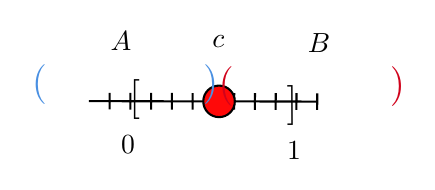
\begin{tikzpicture}[x=0.75pt,y=0.75pt,yscale=-1,xscale=1]
%uncomment if require: \path (0,300); %set diagram left start at 0, and has height of 300

%Straight Lines [id:da035022553384921884] 
\draw    (83,139) -- (193.2,139.2) (93.01,135.02) -- (92.99,143.02)(103.01,135.04) -- (102.99,143.04)(113.01,135.05) -- (112.99,143.05)(123.01,135.07) -- (122.99,143.07)(133.01,135.09) -- (132.99,143.09)(143.01,135.11) -- (142.99,143.11)(153.01,135.13) -- (152.99,143.13)(163.01,135.15) -- (162.99,143.15)(173.01,135.16) -- (172.99,143.16)(183.01,135.18) -- (182.99,143.18)(193.01,135.2) -- (192.99,143.2) ;
%Shape: Circle [id:dp5235472636962212] 
\draw  [fill={rgb, 255:red, 255; green, 9; blue, 9 }  ,fill opacity=1 ] (138.1,139.1) .. controls (138.1,134.9) and (141.5,131.5) .. (145.7,131.5) .. controls (149.9,131.5) and (153.3,134.9) .. (153.3,139.1) .. controls (153.3,143.3) and (149.9,146.7) .. (145.7,146.7) .. controls (141.5,146.7) and (138.1,143.3) .. (138.1,139.1) -- cycle ;

% Text Node
\draw (101,126.9) node [anchor=north west][inner sep=0.75pt]  [font=\Large] [align=left] {[};
% Text Node
\draw (185.07,152.07) node [anchor=north west][inner sep=0.75pt]  [font=\Large,rotate=-179.7] [align=left] {[};
% Text Node
\draw (54,120.1) node [anchor=north west][inner sep=0.75pt]  [font=\Large,color={rgb, 255:red, 74; green, 144; blue, 226 }  ,opacity=1 ]  {$( \ \ \ \ \ \ \ \ \ \ \ \ )$};
% Text Node
\draw (144,121.1) node [anchor=north west][inner sep=0.75pt]  [font=\Large,color={rgb, 255:red, 208; green, 2; blue, 27 }  ,opacity=1 ]  {$( \ \ \ \ \ \ \ \ \ \ \ \ )$};
% Text Node
\draw (92,104.1) node [anchor=north west][inner sep=0.75pt]    {$A$};
% Text Node
\draw (187,105.1) node [anchor=north west][inner sep=0.75pt]    {$B$};
% Text Node
\draw (97,154.1) node [anchor=north west][inner sep=0.75pt]    {$0$};
% Text Node
\draw (177,157.1) node [anchor=north west][inner sep=0.75pt]    {$1$};
% Text Node
\draw (141,106.1) node [anchor=north west][inner sep=0.75pt]    {$c$};


\end{tikzpicture}
\end{center}
\begin{itemize}
    \item Suponga que $1\in B$. Como $I$ es acotado. $\implies A\cap I$ y $B\cap I$ también son acotados. Entonces, por el principio del supremo, $\exists c=sup(A\cap I)>0$ y $c\in A\cup B$
    \item Si $c\in A\implies c<1$\newline 
    $\implies$ como $A$ es abierto $\implies \exists B_r(c)\subset A\implies \exists \alpha \in A\ni c<\alpha (\to\gets)\implies c\not\in A$
    \item Si $c\in B\implies$ como $B$ es abierto. $\implies \exists c_1\in B\ni c_1<c$ y es tal que $[c_1,c]\cap (A\cap i)=\emptyset$ (i.e. $c_1$ es una cota superior de $A\cap I$ y es menor que $c$)($\to\gets$). Entonces, que $c\not\in B(\to\gets)$. 
\end{itemize}
$\implies [0,1]$ es conexo.
\end{proof}

\begin{corollary}
$(0,1)$ es conexo. \marginnote{Si $x$ es un intervalo $\implies x$ es conexo.}
\end{corollary}


\begin{theorem}
$\mathbb{R}^n$ es conexo. 
\end{theorem}

\begin{proof}
Supóngase, por el absurdo, que $A$ y $B$ son una disconexión de $\mathbb{R}^n$
\begin{center}
    

\tikzset{every picture/.style={line width=0.75pt}} %set default line width to 0.75pt        

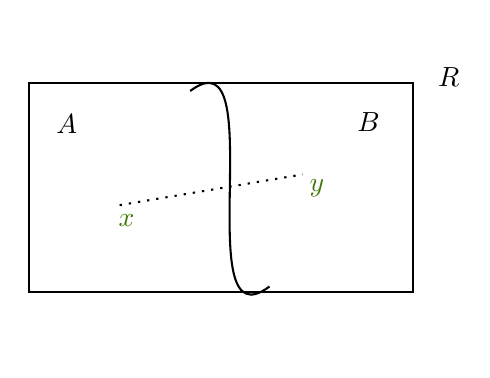
\begin{tikzpicture}[x=0.75pt,y=0.75pt,yscale=-1,xscale=1]
%uncomment if require: \path (0,300); %set diagram left start at 0, and has height of 300

%Shape: Rectangle [id:dp5961020233676221] 
\draw   (50.2,68.2) -- (235.2,68.2) -- (235.2,169) -- (50.2,169) -- cycle ;
%Curve Lines [id:da049078825361805634] 
\draw    (128,72) .. controls (168,42) and (126.2,196.2) .. (166.2,166.2) ;
%Straight Lines [id:da05214217205895033] 
\draw  [dash pattern={on 0.84pt off 2.51pt}]  (94,127) -- (182.2,112.2) ;

% Text Node
\draw (246,59.1) node [anchor=north west][inner sep=0.75pt]    {$\mathbb{R}$};
% Text Node
\draw (62,82.1) node [anchor=north west][inner sep=0.75pt]    {$A$};
% Text Node
\draw (207,81.1) node [anchor=north west][inner sep=0.75pt]    {$B$};
% Text Node
\draw (92,130.1) node [anchor=north west][inner sep=0.75pt]  [color={rgb, 255:red, 65; green, 117; blue, 5 }  ,opacity=1 ]  {$x$};
% Text Node
\draw (184,113.1) node [anchor=north west][inner sep=0.75pt]  [color={rgb, 255:red, 65; green, 117; blue, 5 }  ,opacity=1 ]  {$y$};


\end{tikzpicture}
\end{center}

Sean $x\in A$ y $y\in B$, y considere el segmento de recta que une $x$ con $y$:
$$S=\{(1-t)x+ty:t\in[0,1]\}$$
Sean: $$A_1=\{t\in \mathbb{R}\ni (1-t)x+ty\in A\}$$
$$B_1=\{t\in\mathbb{R}\ni(1-t)x+ty\in B\}$$
\marginnote{$[0,1]$}
$\implies A_1\cap B_1=\emptyset (\to\gets)$, ya que $A_1,B_1$ serían una disconexión de $[0,1]$. Entonces, $\mathbb{R}^n$ es convexo. 
\end{proof}

\begin{remark}
\begin{center}
    

\tikzset{every picture/.style={line width=0.75pt}} %set default line width to 0.75pt        

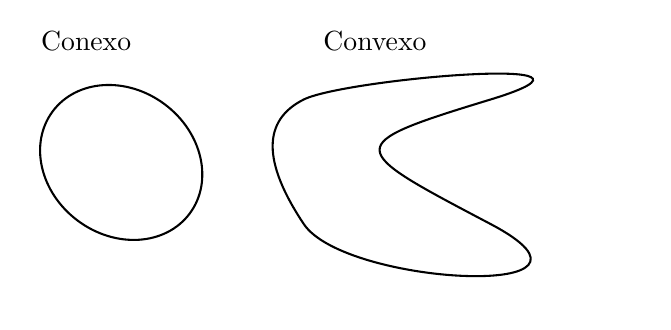
\begin{tikzpicture}[x=0.75pt,y=0.75pt,yscale=-1,xscale=1]
%uncomment if require: \path (0,300); %set diagram left start at 0, and has height of 300

%Shape: Ellipse [id:dp658140374880671] 
\draw   (98.09,156.37) .. controls (79.87,142.76) and (74.48,119.17) .. (86.05,103.69) .. controls (97.62,88.2) and (121.77,86.68) .. (139.98,100.29) .. controls (158.2,113.9) and (163.59,137.48) .. (152.02,152.97) .. controls (140.45,168.46) and (116.31,169.98) .. (98.09,156.37) -- cycle ;
%Shape: Polygon Curved [id:ds3405091393911408] 
\draw   (207,98) .. controls (227,88) and (369.8,75.8) .. (297,98) .. controls (224.2,120.2) and (227.2,121.2) .. (297,158) .. controls (366.8,194.8) and (227,188) .. (207,158) .. controls (187,128) and (187,108) .. (207,98) -- cycle ;

% Text Node
\draw (79,63.9) node [anchor=north west][inner sep=0.75pt]   [align=left] {Conexo};
% Text Node
\draw (215,63.9) node [anchor=north west][inner sep=0.75pt]   [align=left] {Convexo};


\end{tikzpicture}
\end{center}
\end{remark}

\begin{theorem}
Los únicos conjuntos abiertos y cerrados de $\mathbb{R}^n$ son $\emptyset$ y $\mathbb{R}^n$
\end{theorem}
\begin{proof}
Supóngase, por el absurdo, que $A\subset \mathbb{R}^n$, $A\neq \emptyset$ y $A\neq \mathbb{R}^n$, es abierto y cerrado de $\mathbb{R}^n$. Como $A$ es cerrado $\implies A^c=B$ es abierto. 
$\implies A\neq \emptyset \implies B\neq \emptyset,A\cap B=\emptyset$ y $A\cup B=\mathbb{R}^n$. $\implies A$ y $B$ forman una disconexión de $\mathbb{R}^n(\to\gets)$. $\implies$ los únicos abiertos y cerrados de $\mathbb{R}^n$ son $\emptyset$ y $\mathbb{R}^n$ 
\end{proof}

\begin{theorem}
Un subconjunto de $\mathbb{R}$ es conexo ssi es un intervalo. 
\end{theorem}
\begin{theorem}
\begin{itemize}
    \item $(\gets)$ A probar cada intervalo de $\mathbb{R}$ es un conexo (ver prueba de: $[0,1]$ es conexo=.
    \item $(\to)$ Sea $C\subset \mathbb{R}$, conexo. A probar: $C$ es un intervalo. Sean $a,b\in C\ni a<b$ y sea $x\in\mathbb{R}\ni a<x<v$. A probar: $x\in C$\begin{center}
        

\tikzset{every picture/.style={line width=0.75pt}} %set default line width to 0.75pt        

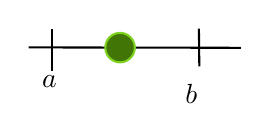
\begin{tikzpicture}[x=0.75pt,y=0.75pt,yscale=-1,xscale=1]
%uncomment if require: \path (0,300); %set diagram left start at 0, and has height of 300

%Straight Lines [id:da6796265049147991] 
\draw    (89,141) -- (191.2,141.2) ;
%Straight Lines [id:da07800145146886805] 
\draw    (100.2,132.2) -- (100.2,152.2) ;
%Straight Lines [id:da617799668252107] 
\draw    (171,132) -- (171.2,150.2) ;
%Shape: Circle [id:dp7757914759860494] 
\draw  [color={rgb, 255:red, 126; green, 211; blue, 33 }  ,draw opacity=1 ][fill={rgb, 255:red, 65; green, 117; blue, 5 }  ,fill opacity=1 ] (125.9,141.1) .. controls (125.9,137.18) and (129.08,134) .. (133,134) .. controls (136.92,134) and (140.1,137.18) .. (140.1,141.1) .. controls (140.1,145.02) and (136.92,148.2) .. (133,148.2) .. controls (129.08,148.2) and (125.9,145.02) .. (125.9,141.1) -- cycle ;

% Text Node
\draw (94,153.1) node [anchor=north west][inner sep=0.75pt]    {$a$};
% Text Node
\draw (163,157.1) node [anchor=north west][inner sep=0.75pt]    {$b$};


\end{tikzpicture}
    \end{center}
    Si $x\not\in C\implies (-\infty,c)$ y $(x,\infty)$ formar una disconexión de $c$. 
\end{itemize}
\end{theorem}